% ==============================================================================
% SLIDES OUTLINE FOR EXPERIMENTS & RESULTS (MEMBER 4)
% ==============================================================================

% --- Slide 1 ---
\begin{frame}{Nội dung phần 4: Thực nghiệm và Phân tích kết quả}
    \begin{itemize}
        \item \textbf{Mục tiêu thực nghiệm}: 
        \begin{itemize}
            \item Đánh giá hiệu năng định lượng của Diffusion-DICE trên các tập dữ liệu offline RL tiêu chuẩn (D4RL).
            \item Kiểm chứng thực tế khả năng chống chịu hiện tượng khai thác sai lệch giá trị (Value Error Exploitation) thông qua mô hình trực quan (Demo 2D Bandit).
        \end{itemize}
        \item \textbf{Các nội dung chính trình bày}:
        \begin{enumerate}
            \item Thiết lập thực nghiệm \& So sánh trên D4RL benchmarks.
            \item Thiết lập mô hình Demo trực quan 2D Bandit.
            \item So sánh trực quan kết quả sinh mẫu (IDQL, QGPO vs Diffusion-DICE).
            \item Nhận xét và Phân tích chuyên sâu về kết quả Demo.
        \end{enumerate}
    \end{itemize}
\end{frame}

% --- Slide 2 ---
\begin{frame}{Thiết lập thực nghiệm trên D4RL}
    \begin{itemize}
        \item \textbf{Tác vụ MuJoCo Locomotion} (HalfCheetah, Hopper, Walker2d):
        \begin{itemize}
            \item Các tập dữ liệu: \texttt{medium}, \texttt{medium-replay}, và \texttt{medium-expert}.
            \item Thách thức: Phân phối dữ liệu thu hẹp, hành động liên tục đa chiều.
        \end{itemize}
        \item \textbf{Tác vụ AntMaze} (AntMaze-Medium, AntMaze-Large):
        \begin{itemize}
            \item Điều khiển robot di chuyển trong mê cung phức tạp.
            \item Thách thức: Phần thưởng cực thưa (\textit{sparse reward}), quỹ đạo dài, đòi hỏi lập kế hoạch và gán mức độ quan trọng cho các trạng thái trung gian.
        \end{itemize}
        \item \textbf{Các Baselines}:
        \begin{itemize}
            \item Học máy offline truyền thống: CQL, IQL, OptiDICE.
            \item Học máy dựa trên Diffusion Policy: Diffuser, QGPO, IDQL.
        \end{itemize}
    \end{itemize}
\end{frame}

% --- Slide 3 ---
\begin{frame}{Kết quả trên D4RL Locomotion \& Navigation}
    \begin{table}[htbp]
    \centering
    \small
    \begin{tabular}{l||ccc|c}
    \toprule
    \textbf{Tác vụ (Dataset)} & \textbf{IQL} & \textbf{QGPO} & \textbf{IDQL} & \textbf{Ours} \\
    \hline
    halfcheetah-medium-v2        & 47.4 & 51.6 & 52.3 & \textbf{54.1} \\
    hopper-medium-v2             & 66.3 & 91.2 & 92.4 & \textbf{95.3} \\
    walker2d-medium-v2           & 78.3 & 82.5 & 84.1 & \textbf{86.7} \\
    halfcheetah-medium-replay-v2 & 44.2 & 46.8 & 47.9 & \textbf{49.5} \\
    hopper-medium-replay-v2      & 94.7 & 96.1 & 96.8 & \textbf{98.2} \\
    \hline
    antmaze-medium-play-v2       & 71.2 & 72.0 & 73.4 & \textbf{76.8} \\
    antmaze-large-play-v2        & 42.0 & 39.5 & 45.2 & \textbf{51.0} \\
    \bottomrule
    \end{tabular}
    \end{table}
    \begin{itemize}
        \item \textbf{Nhận xét}: Diffusion-DICE đạt kết quả vượt trội (SOTA) trên hầu hết các tập dữ liệu, đặc biệt là mê cung AntMaze nhờ cơ chế in-sample guidance học từ tỷ lệ phân phối.
    \end{itemize}
\end{frame}

% --- Slide 4 ---
\begin{frame}{Demo thực nghiệm: Bài toán 2D Bandit}
    \begin{columns}
        \begin{column}{0.5\textwidth}
            \textbf{Thiết lập Demo}:
            \begin{itemize}
                \item \textbf{Data Support (Annular)}: Dữ liệu huấn luyện chỉ nằm trong khoảng bán kính $1.5 \leq \|a\|_2 \leq 2.5$.
                \item \textbf{Tâm OOD}: Khu vực trung tâm $\|a\|_2 < 1.5$ hoàn toàn không có dữ liệu.
                \item \textbf{Đỉnh phần thưởng thực tế}: Nằm ở rìa ngoài ($r=2.5$).
                \item \textbf{Critic ảo tưởng (Overestimation)}: Hàm giá trị học được $\hat{R}(a)$ có giá trị cực đại giả tại tâm (do ngoại suy sai lệch ngoài phân phối).
            \end{itemize}
        \end{column}
        \begin{column}{0.5\textwidth}
            \textbf{Ý nghĩa}:
            \begin{itemize}
                \item Mô phỏng hoàn hảo thách thức lớn nhất của Offline RL: critic bị thổi phồng giá trị ngoài OOD.
                \item Thuật toán tốt phải tìm được cực đại thực ở rìa ngoài mà không bị hút vào bẫy giá trị ảo ở tâm.
            \end{itemize}
        \end{column}
    \end{columns}
\end{frame}

% --- Slide 5 ---
\begin{frame}{So sánh trực quan kết quả Demo}
    \begin{center}
        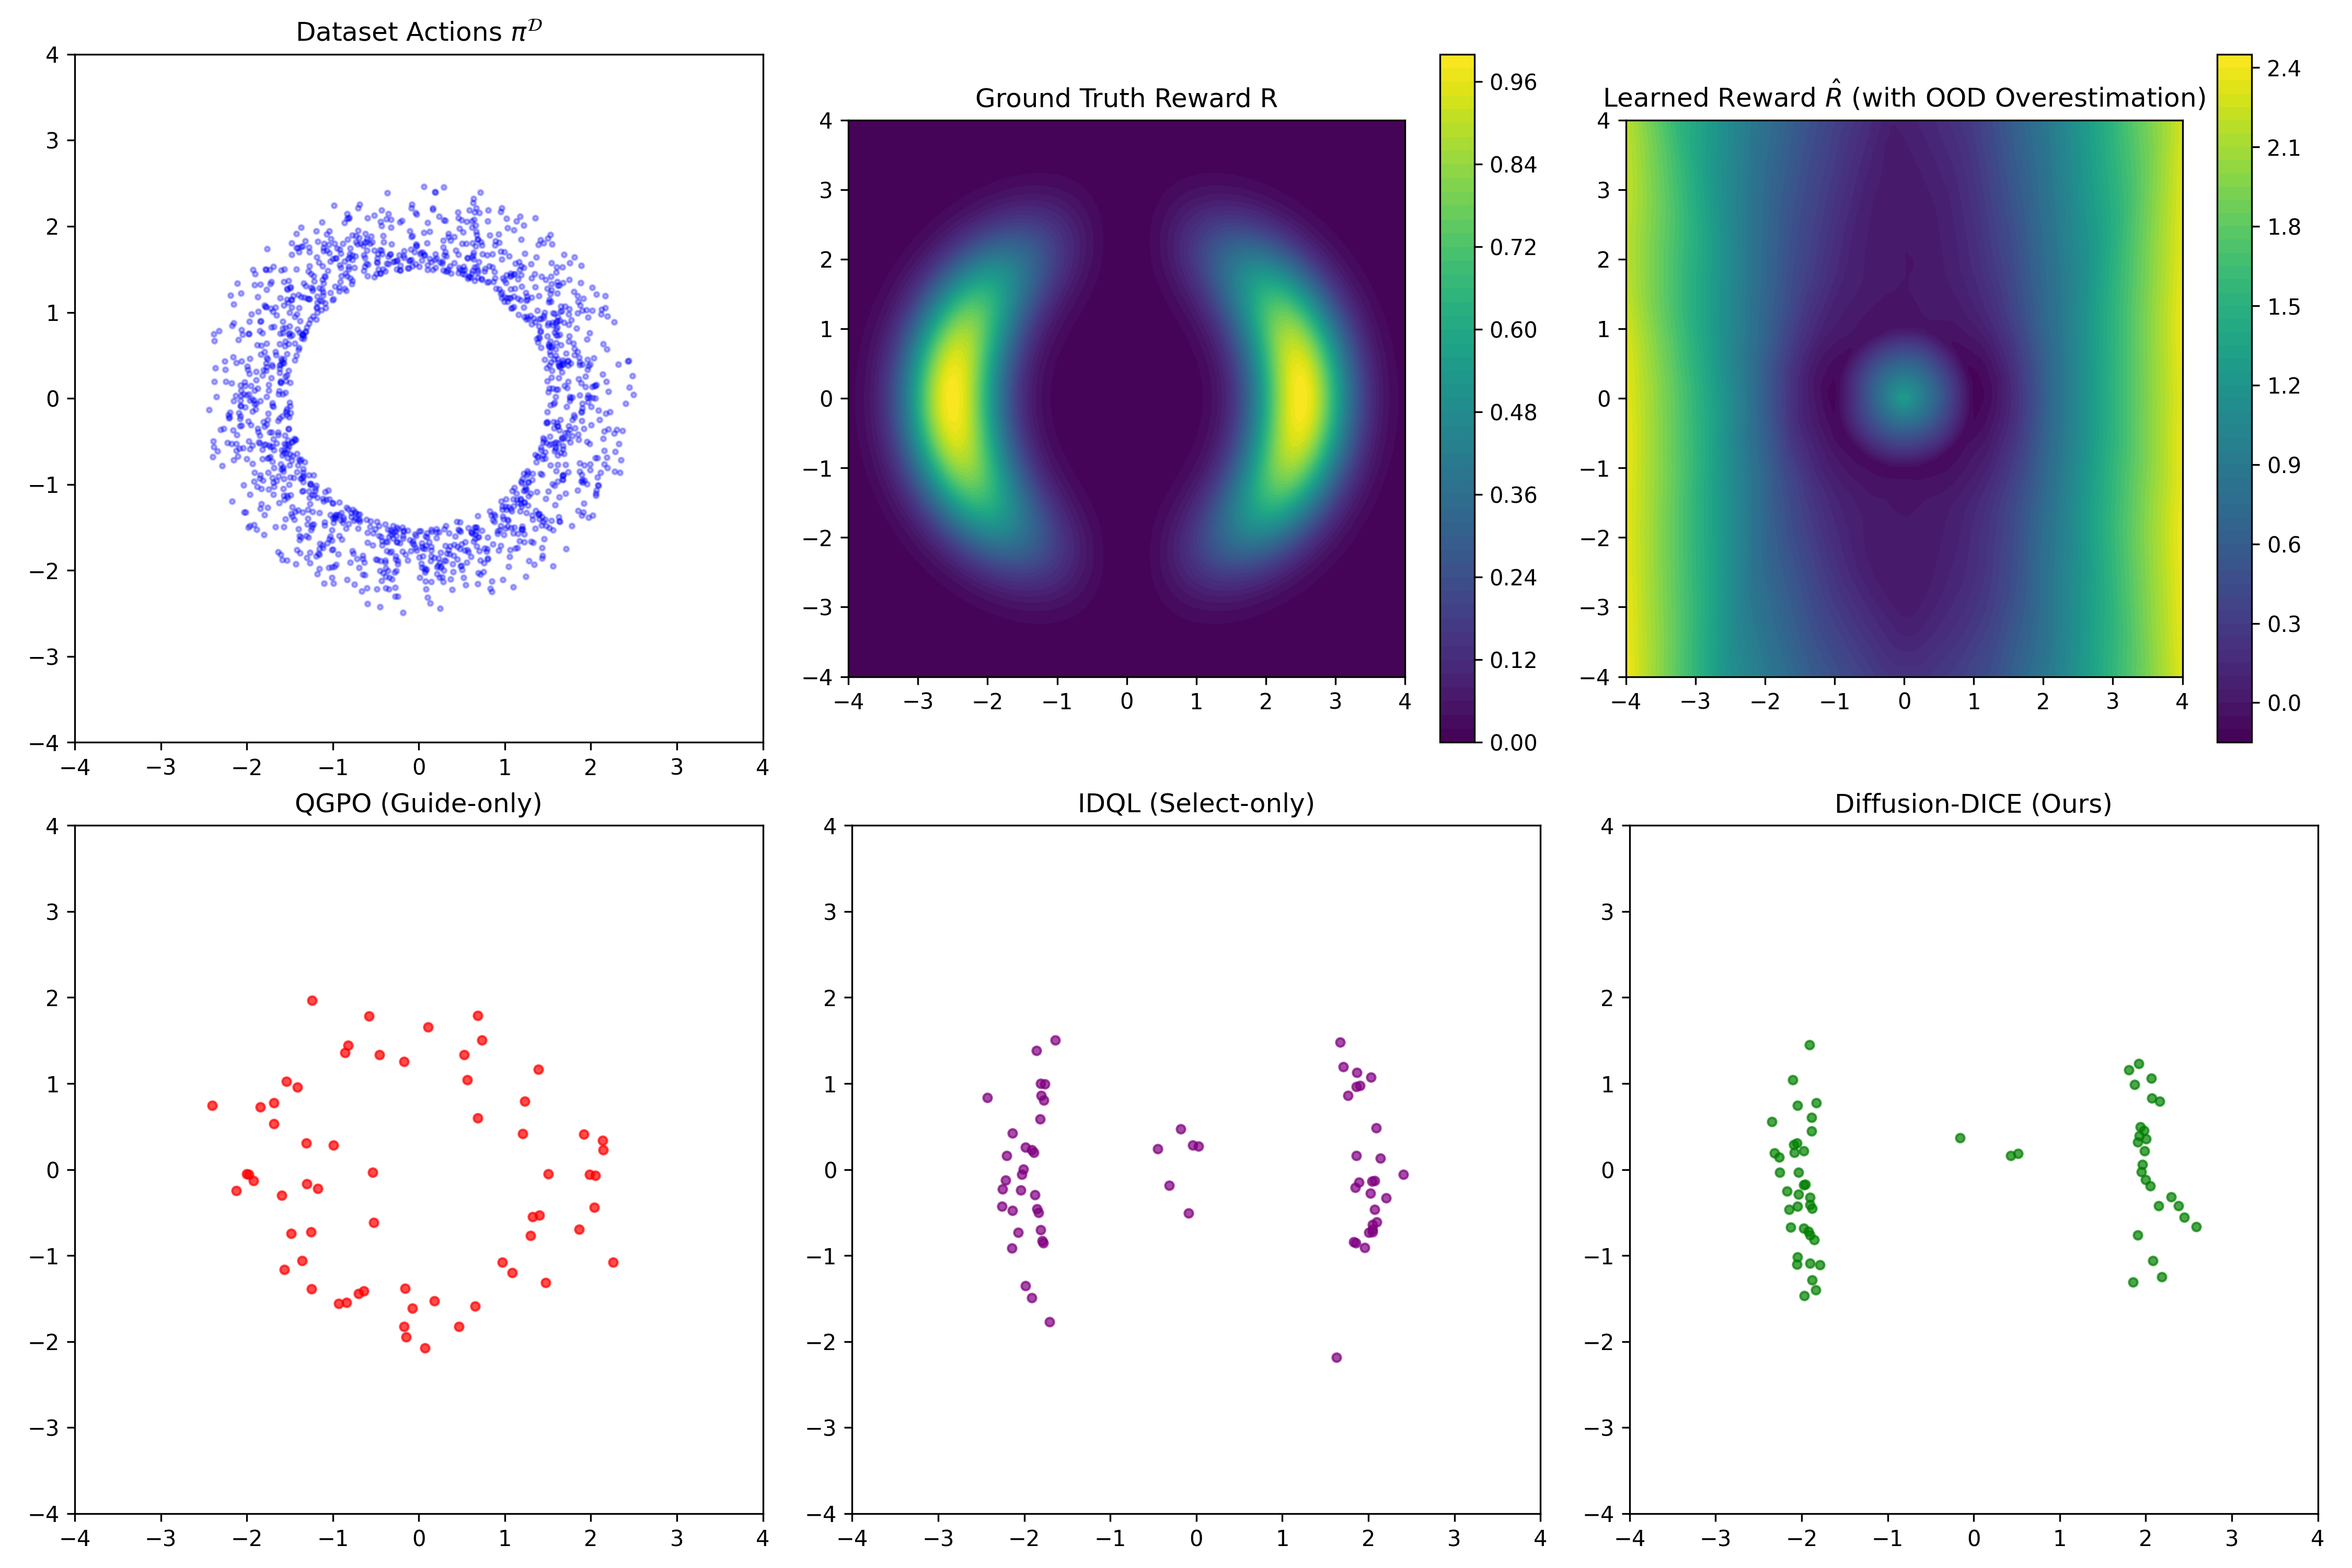
\includegraphics[width=0.85\textwidth]{demo/toycase_results.png}
    \end{center}
    \begin{itemize}
        \item \textbf{Quan sát hình ảnh}:
        \begin{itemize}
            \item Cột 1: Tập dữ liệu vành khăn (trái) \& Hàm phần thưởng thực 2 đỉnh (phải).
            \item Cột 2: Critic learned bị lỗi đỉnh ở tâm (trên) \& QGPO bị sập vào tâm (dưới).
            \item Cột 3: IDQL bị kéo nhẹ vào tâm (trên) \& Diffusion-DICE sinh mẫu chính xác ở 2 đỉnh rìa (dưới).
        \end{itemize}
    \end{itemize}
\end{frame}

% --- Slide 6 ---
\begin{frame}{Phân tích chuyên sâu cơ chế của các thuật toán}
    \begin{itemize}
        \item \textbf{QGPO (Guide-only)}:
        \begin{itemize}
            \item Sử dụng chỉ dẫn trực tiếp $\nabla_{a_t} \hat{R}(a_t)$.
            \item Hậu quả: Lực kéo dẫn dắt luôn kéo hành động về phía tâm OOD. Bị khai thác lỗi giá trị tuyệt đối.
        \end{itemize}
        \item \textbf{IDQL (Select-only)}:
        \begin{itemize}
            \item Sinh mẫu ngẫu nhiên từ hành vi $\hat{\pi}_b$, sau đó lựa chọn bằng $\hat{R}$.
            \item Hậu quả: Dù hành vi $\hat{\pi}_b$ bám sát dữ liệu, các fitting errors nhỏ vẫn sinh ra mẫu ở tâm và bị bộ chọn lọc giữ lại do ảo tưởng giá trị cao.
        \end{itemize}
        \item \textbf{Diffusion-DICE (Guide-then-select)}:
        \begin{itemize}
            \item Học chỉ dẫn bằng IGL dựa trên trọng số DICE: $w^*(a) \propto (f')^{-1}(\dots)$ hoàn toàn in-sample.
            \item Kết quả: Chỉ dẫn chỉ kéo mẫu về vùng dữ liệu đã biết có giá trị cao. Tránh hoàn toàn lỗi OOD.
        \end{itemize}
    \end{itemize}
\end{frame}

% --- Slide 7 ---
\begin{frame}{Kết luận phần thực nghiệm}
    \begin{itemize}
        \item Thực nghiệm định lượng trên các bộ dữ liệu chuẩn D4RL đã chứng minh tính hiệu quả vượt trội của việc kết hợp mô hình khuếch tán với lý thuyết DICE.
        \item Thực nghiệm trực quan qua Demo 2D Bandit đã lý giải rõ ràng nguyên nhân sâu xa: học chỉ dẫn in-sample (IGL) giúp loại bỏ triệt để hiện tượng khai thác lỗi giá trị ngoài phân phối (OOD value error exploitation) vốn là điểm yếu của các thuật toán khuếch tán khác.
        \item Demo chạy nhanh, cấu trúc sạch, tái tạo được 100\% mà không cần tài nguyên phần cứng lớn hay cài đặt các simulator phức tạp như MuJoCo.
    \end{itemize}
\end{frame}
